\setchapterpreamble[u]{\margintoc}
\chapter{Approssimazioni}
\labch{approx}

\section{Introduzione}

Le approssimazioni di funzioni rivestono un ruolo fondamentale in ambito scientifico,
specialmente nella fisica computazionale, dove spesso non è possibile risolvere
esattamente le equazioni che descrivono i fenomeni fisici.

Queste approssimazioni permettono di semplificare funzioni complesse attraverso
metodi numerici, rendendo più accessibile la loro analisi e il calcolo delle
soluzioni.
Tali tecniche consentono di ottenere stime accurate di grandezze fisiche che
altrimenti sarebbero difficili da trattare analiticamente, con una precisione
dipendente dalla complessità del modello e dalla quantità di risorse computazionali
disponibili.

Alcuni dei metodi più comuni includono l'approssimazione polinomiale;
le serie di Taylor, argomento di questa sezione; o tecniche come l'interpolazione
che sarà l'argomento della quinta sezione.

\section{Esercizi}


\subsection{Funzione esponenziale}

\paragraph{Nozioni teoriche}

La funzione esponenziale è esprimibile in serie di McLaurin come:

$$
	e^x = \sum_{n=0} \frac{x^n}{n!} + \epsilon
$$

dove $\epsilon$ rappresenta l'errore commesso nell'approssimare la funzione:

$$
	\epsilon \approx \frac{x^{n+1}}{(n+1)!}
$$

ove $n$ è il grado della serie di Taylor.

\paragraph{Implementazione e osservazioni}

% file necessari
\subparagraph{File necessari} sorgente: \texttt{exp\_approx.c}, dati: \texttt{exp\_approx\_$n$.dat} \\ $n = 1, 2, 3, 4$

\begin{marginfigure}
	\centering
	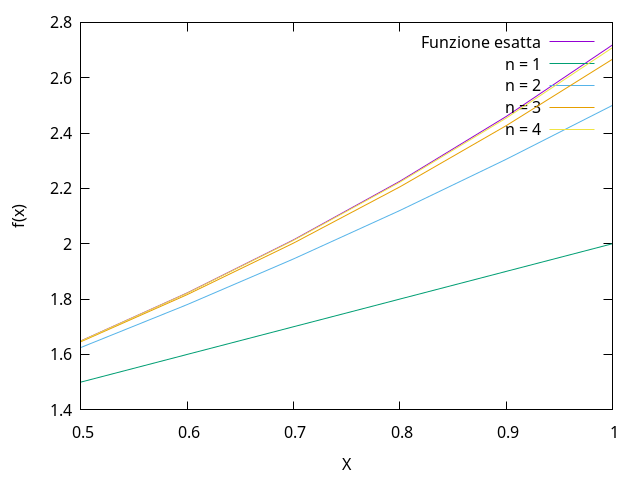
\includegraphics[width=1.5\textwidth]{exp_confront.png}
	\caption{Confronto tra funzione esponenziale e la n-esima approssimazione}
	\labfig{expfunc}
\end{marginfigure}


\begin{marginfigure}
	\centering
	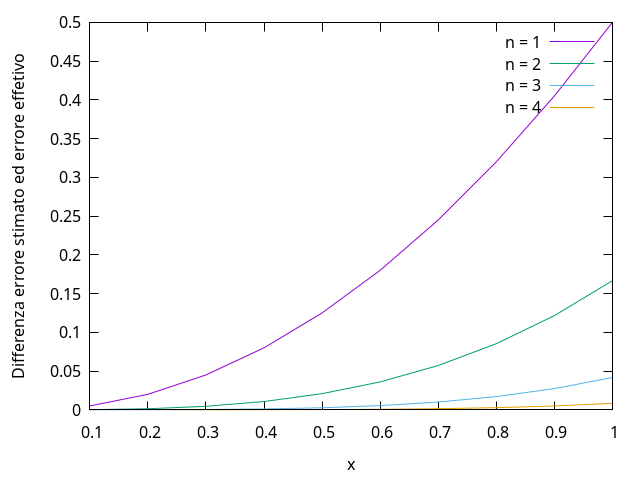
\includegraphics[width=1.5\textwidth]{error_diff_n.png}
	\caption{Differenza tra errore teorico ed errore ottenuto}
	\labfig{errordiff}
\end{marginfigure}

La funzione esponenziale ottenuta approssimando si può osservare in \reffig{expfunc}.

\begin{enumerate}
	\item L'errore scala effettivamente come $\frac{x^{n+1}}{(n+1)!}$ per valori
	      vicini a 0 e per valori di n maggiori, come si può osservare in \reffig{errordiff}.

	\item Sempre dalla \reffig{errordiff} si può notare come l'errore aumenti all'allontanarsi
	      da x = 0 e cominci a differire dall'errore teorico.
	      Ciò si intuscisce studiando la condizione per cui continui $\epsilon_{teorico} \approx \epsilon_{reale}$ è
	      soddisfatta: $$\epsilon_{teorico} \ll 1$$ La condizione dipende
	      da $n$ e $x$ per valori bassi di $n, x^n$ prevale sul fattoriale e la differenza
	      da $\epsilon_{teorico}$ è maggiormente visibile. Come si può vedere in \reffig{errordiff}
	      per $n = 4$ e l'errore tende a 0 molto più velocemente.

\end{enumerate}

% NOTE: la differenza dall'errore teorico aumenta all'allontanarsi da x = 0 poiche'
% la serie di taylor e' stata espansa in x = 0

\subsection{Problema di Basilea}

\paragraph{Nozioni teoriche}

Il problema di Basilea consiste nel calcolare il valore della serie armonica generalizzata:

$$
	S(N) = \sum_{n=1}^{N} \frac{1}{n^2} \xrightarrow{N \to \infty} \zeta(2) = \frac{\pi^2}{6}
$$

\paragraph{Osservazioni e conclusioni}

\subparagraph{Singola precisione}

I valori ottenuti per numeri a singola precisione sono:
% due valori, somma inversa e somma diretta

$$
	S_{incr}(N) \approx \mathtt{1.6447253} \quad \text{per } N = 6000
$$

$$
	S_{inv}(N) \approx \mathtt{1.6447674} \quad \text{per } N = 6000
$$

\begin{figure}[H]
	%	\centering
	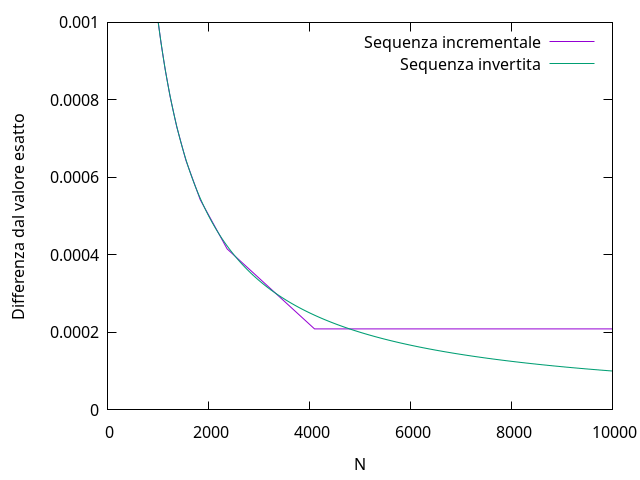
\includegraphics[width=1.5\columnwidth]{seq_inv_sum_error.png}
	\caption{$|S(N) - \pi^6 / 2|$ per valori grandi di N, si nota un singolare
		andamento della somma a partire da valori $ x \approx 4000$, \textbf{la
			stessa cosa non succede invece per numeri a doppia precisione}}
	\labfig{sumerr}
\end{figure}

Il risultato è spiegabile in maniera equivalente a \ref{sec:propagation}: l'ordine
della somma conta nella propagazione di errori in numeri a virgola mobile. Infatti:
\begin{itemize}
	\item Nella somma incrementale, il valore di partenza è $1/1^2 = 1$ (il valore
	      \textit{più grande} della somma con errore $\epsilon \approx 10^{-7}$),
	      dato che la somma si propaga con gli errori assoluti degli addendi,
	      considerando $N = 4000$:

	      $$\epsilon_{tot} \approx N \epsilon \approx 4 \cdot 10^{-4}$$

	      Che è circa lo stesso ordine di grandezza in cui inizia l'andamento costante
	      della somma. Per $N > 4000$ la somma perde le informazioni su numeri piccoli
	      poichè l'errore propagato è maggiore del valore sommato.

	\item La somma invertita, invece, inizia con il valore più piccolo della serie,
	      per esempio $1/4000^2 \approx 6.25 \cdot 10^{-8}$, e propaga con errori sempre maggiori
	      ma inferiori alle cifre significative del valore successivo (più grande).
	      Ciò comporta che la perdita di informazioni non è abbastanza significativa
	      per causare errori di arrotondamento notevoli.
\end{itemize}
\subparagraph{Doppia precisione}

In doppia precisione l'errore macchina è ancora minore e l'effetto diventa trascurabile
subentrano ulteriori errori non causati dalla precisione del numero ma da limiti 
del programma scritto o del compilatore/interprete utilizzato.

In conclusione, si sottilinea, come nel capitolo precedente, l'importanza di considerare
l'ordine della somma e la precisione del calcolo in problemi numerici.









